\chapter{Introduction}
%labels will help you to reference to certain images, tables, chapters, section, and so on...
\label{introduction}
This chapter presents an explanation about what has served as motivation for this thesis. What else is provided are the approach for solving the issue as well as the aims of the work. At the end of the chapter, the structure is defined.

%###################################################################################
%###################### Motivation          ########################################
%###################################################################################
\section{Motivation}
In recent times, the amount of interest in a cooperative environment for autonomous vehicles and infrastructure has increased and there are many researches on this topic \cite{ cvis_article_one, cvis_article_two}. Its main goal is to increase safety, decrease number of accidents and improve efficiency of city traffic. In order to achieve this it must be guaranteed that the self-steering vehicles are aware of their surroundings during the whole ride \cite{onboard_sensors}.

Nowadays, the cars with the highest level of autonomy\footnote{\url{https://www.auto123.com/en/news/vehicle-autonomy-levels-explained/64372}, visited on 13/11/2022} integrate a combination of sensors like radar, Light Detection and Ranging (LiDAR) and camera systems to be able to perceive other traffic participants \cite{autonomous_cars_sensors}. In spite of their widespread adoption in the automobile industry for guaranteeing a high level of safety and driving facilitation, on-board sensors have their drawbacks like limited visibility and decreased field of perception. Another issue is that vehicle-integrated sensors cannot have a clear estimation when there is an object that impedes their field of view (FoV). Thus, the use of stationary sensors in a city infrastructure is beneficial for providing more reliable and accurate information \cite{roadside_lidar}. Moreover, placement of sensors in the road area expands significantly the vehicle's range of view and contributes to safer and congestion-free roads. Unlike other sensors, cameras are cheaper and much easier to maintain\footnote{\url{https://www.autopilotreview.com/lidar-vs-cameras-self-driving-cars/}, visited on 13/11/2022}. Another advantage is that they are capable of seeing the world like a human being would do, which is of utmost importance in object detection and tracking algorithms \cite{camera_object_detection}. The highly researched camera technology and its features are main reasons for this thesis to focus on its usage for aiding a robust autonomous driving.

Real-world experiments for investigating which sensor placement is optimal should always be planned precisely and require careful preparation to ensure that various factors could not impact the results. In addition, conducting tests in the real world results in more costs and effort to reproduce a specific scenario. For the purpose of reducing costs and considering a greater range of camera positioning options, this work relies on the 3D autonomous driving simulator CARLA\footnote{\url{https://carla.org/}, visited on 13/11/2022}. It is used for generating simulated data samples for different camera placements, which is then evaluated by using heatmaps and the results are summarized.

% DELETEME: Example for a chain: Mobile communication gets increasingly popular in the world (CITE sales on mobile communication infrastructure, mobile phones, or increasing number of mobile phones contracts). $\rightarrow$ Especially smartphones, which represent the next generation cellular phone (CITE), get more and more used for communicating not only with other people but also for connecting to the Internet for using various services (CITE). $\rightarrow$ Smartphone are comprehensive cellular phones that provide additional functionality due to their increased connection and processing capabilities (CITE). $\rightarrow$ Most smartphones offer an online application store for adding software to the devices which helps the users to customize their devices according to their needs, e.g. Android Market\footnote{\url{http://market.android.com}, visited on 05/08/2011}. $\rightarrow$ One problem about installing third-party software is that not all software try to help the user; $\rightarrow$ software with malicious intentions, so-called malicious software (malware), can be a severe threat to smartphone users. Some malware delete files (EXAMPLE + CITE or footnote with URL) or even destroy devices (EXAMPLE + CITE or footnote with URL). $\rightarrow$ More and more smartphone malware appeared in the last years (CITE). $\rightarrow$ Signature-based approaches work efficiently on known malware (CITE) but face serious drawbacks regarding unknown malware. $\rightarrow$ Oberheide et al.~\cite{oberheide:2008:cloudav} state that virus engines need an average time of 48 days until their databases get updated to be able to detect a certain unknown malware. $\rightarrow$ This in turn means that smartphone users stay unprotected for this time, which can be seen as a severe threat. $\rightarrow$ Therefore, approaches are needed that are capable of detecting unknown malware for protecting the users against such threats.
% DELETEME: This example showed how one could argue that alternative approaches for malware detection is required. The length of the motivation depends on the topics handled and can of course be longer. The principle I am describing is also shown on Figure~\ref{fig:writing}

% \begin{figure}
% \centering
% 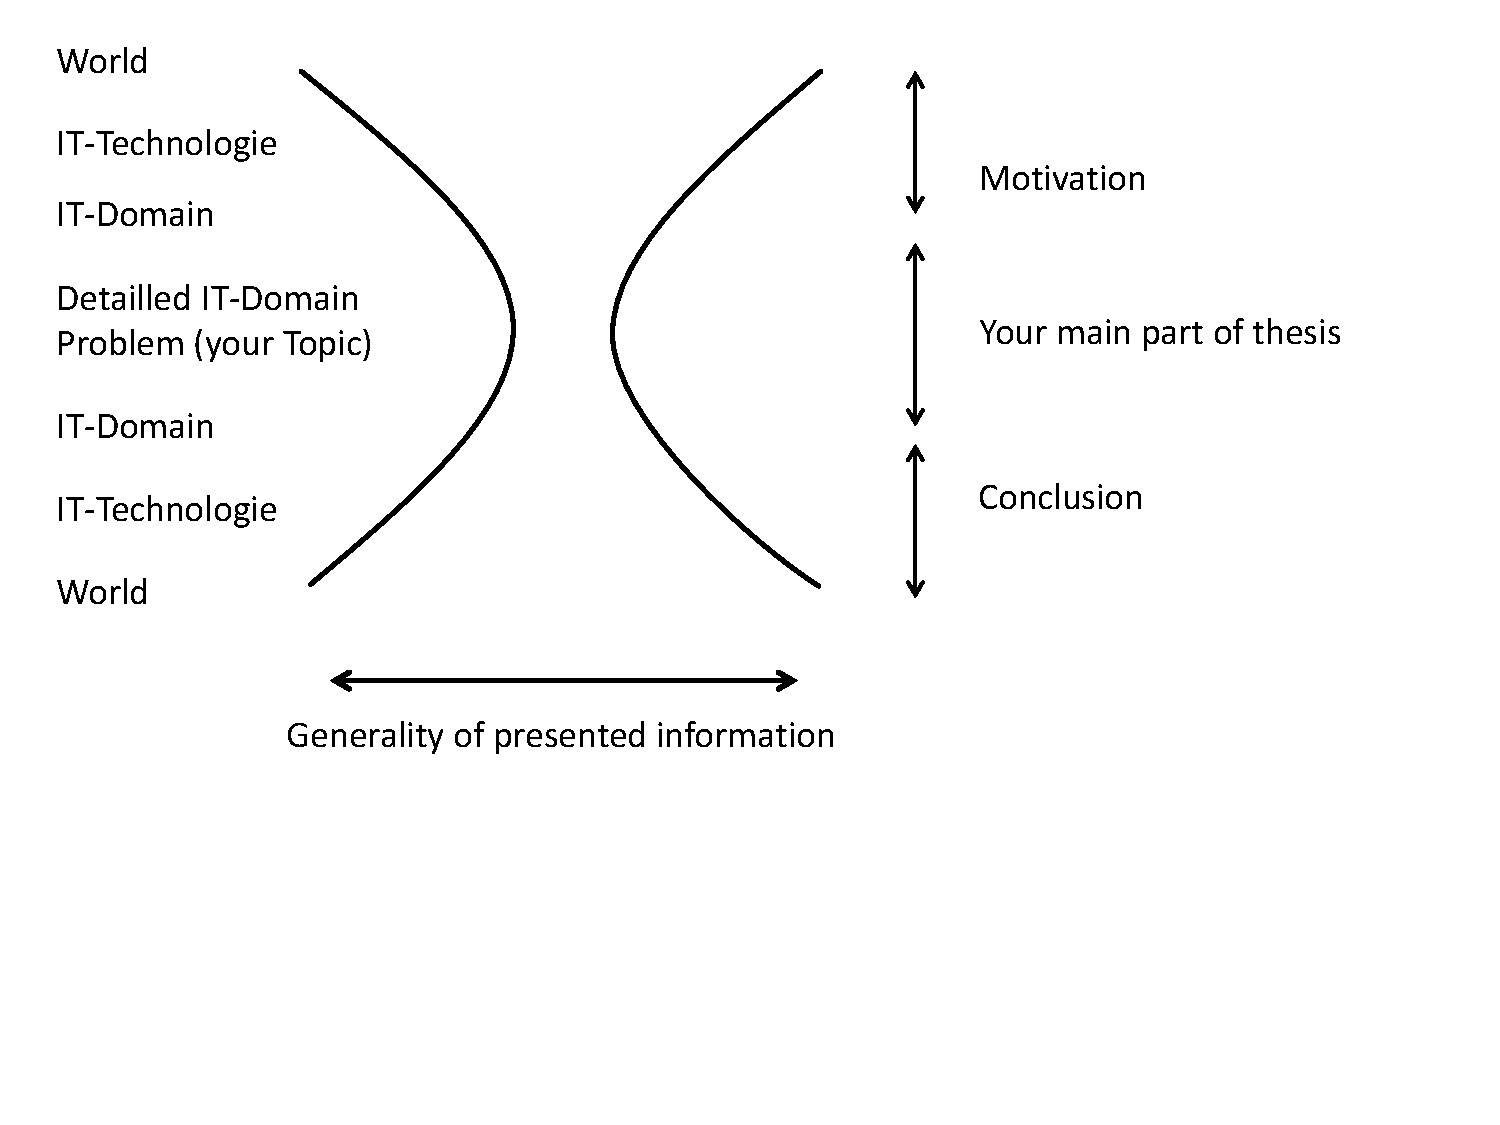
\includegraphics[width=0.9\textwidth]{template/writing}
% \caption[Information Generality]{This images illustrates how generality of information could be handled in a thesis. In your motivation you should start from a very broad view on the topic. Then you should get more precise with every statement until you reach the actual problem you are addressing. You should do vice-versa in your conclusion, starting with the problem that you addressed and getting broader until you can write about the meaning of your results to the (IT-)world.\label{fig:writing}}
% \end{figure}


%###################################################################################
%###################### Approach and Goals  ########################################
%###################################################################################
\section{Approach and Goals}
% DELETEME: In this section, you should cleary describe your approach that you are following in order to solve the underlaying problem of your thesis. Additionally, you should clearly state the goals of your work. This will not only help you supervizor to understand what you are doing, it will also help you to be sure on which topic you should evaluate.

The main goal of this thesis is to estimate an optimal camera position and its configuration using a simulated environment, where no real-world limitations occur. For the approach all simulations are executed on a junction of four roads as it is considered being the one with most conflict points by the European Road Safety Observatory\footnote{\url{https://www.dacota-project.eu/Links/erso/knowledge/Content/15_road/junctions.html}, visited on 13/11/2022}. We place a stationary monocular camera in the infrastructure in such positions that a greater range of interest (ROI) lands in the sensor's FoV. During the experiments, we spawn two static vehicles on all possible points, which the junction contains and which are captured on the image plane. As a following step, we apply a mathematical model - Occlusion Degree Model (ODM) \cite{occlusion_degree_model} - for estimation of the percentage, which expresses the part of the target vehicle that is occluded by the occluder vehicle. With the help of the model and an instance segmentation camera \cite{instance_segmenatation_cam}, this work estimates the efficiency of different camera placement options. On every captured image the pixels containing vehicles are coloured based on their ID in the Unity Engline\footnote{\url{https://www.unrealengine.com/de/blog/welcome-to-unreal-engine-4}, visited on 14/11/2022}. Having this data, we extract the covered area of the target vehicle after each spawn and summarize the results in a heatmap. Finally, we compare the results and select the ones, which perceived as less occlusion as possible in various vehicle placement combinations. 
\newpage

%###################################################################################
%###################### Structure of the Thesis ####################################
%###################################################################################
\section{Structure of the Thesis}
% DELETEME: This section does not require eloquent writing. It is just a presentation of what you will handle in each chapter starting with Chapter~\ref{background}.

% DELETEME: Example: This thesis is structured as follows. In Chapter~\ref{background}, we discuss essential background related to the thesis topic. (SOME MORE SENTENCES). Chapter~\ref{mainone} represents a detailed analysis of the problem that will be addressed. In particular, (SOME MORE SENTENCES). In Chapter~\ref{maintwo}, our solution is presented. This solution covers ... (SOME MORE SENTENCES). Chapter~\ref{evaluation} evaluates our solution basing on our specified goals. (SOME MORE SENTENCES). In Chapter~\ref{conclusion}, we conclude. Chapter~\ref{appendices} gives additional related information on the topic of this thesis.

\myworries{HAVE TO UPDATE THE WHOLE INTRODUCTION}

The next chapters of this thesis are structured as follows: 
\begin{itemize}
    \item Chapter \ref{background} talks about scientific information regarding camera, etc.
    \item Chapter \ref{mainone} reveals some state-of-the-art methods for sensor placement, etc.
    \item In chapter \ref{maintwo} the problem that this thesis is concerned with and an approach for solving it are presented.
    \item Chapter \ref{evaluation} introduces the results of the conducted experiments and delivers insight into how they were evaluated.
    \item In the \ref{conclusion} chapter we summarize the outcome of our experiments and discuss the possible tasks for a future work on this issue.
\end{itemize} 
